% !TeX spellcheck = en_GB
\documentclass[11pt]{enstaPRE}

%% Useful packages
\usepackage{amsthm}
\usepackage{amsmath}
\usepackage{amssymb}
\usepackage{graphicx}
\usepackage{caption}
\usepackage{dsfont}

\logo{logos/Leeds.png}
\specialite{SIM}
\annees{2017-2018}
\titre{Numerical schemes for SDEs with distributional coefficients}
\soustitre{}
\illustration{images/maths.jpg}
\confidentialite{Non-confidential report and publishable on Internet}
\auteur{Maximilien Germain}
\promotion{2019}
\tuteurENSTA{Francesco Russo}
\tuteurOrganisme{Elena Issoglio, Tiziano de Angelis}
\dateDebut{05-14-2018}
\dateFin{08-03-2018}
\organisme{University of Leeds}
\adresseOrganisme{Woodhouse Lane\\Leeds\\LS2 9JT\\United Kingdom}

\newtheorem{defi}{Definition}
\newtheorem{theo}{Theorem}
\newtheorem{lem}[theo]{Lemma}
\newtheorem{cor}[theo]{Corollary}
\newtheorem{Pro}[theo]{Proposition}
\newtheorem{ex}{Example}
\newtheorem{rem}{Remark}

\newcommand{\de}[2]{\frac{\mathrm{d} #1}{\mathrm{d} #2}}
\newcommand{\norme}[1]{\left\Vert #1\right\Vert}
\newcommand{\R}{\mathbb{R}}
\newcommand{\Z}{\mathbb{Z}}
\newcommand{\N}{\mathbb{N}}
\newcommand{\E}{\mathbb{E}}
\newcommand\gts[1]{\og#1\fg}
\newcommand{\di}{\mathrm{d}}
    
\begin{document}

\couverture

\pageConfidentialite{This present document is not confidential. It can be communicated outside in
paper format or distributed in electronic format.}

\partb{Acknowledgment}

Elena, Tiziano, Francesco.

\partb{Abstract}
This project studies an approximation method of a stochastic differential equation with distributional drift. It adapts and applies the usual Euler-Marayuma scheme to a new class of problems with irregular coefficients. We prove the convergence of our algorithm and study the numerical results obtained in the special case of a fractional brownian motion path as a drift.

\paragraph{}
\textbf{Keywords and phrases:} Stochastic differential equations; distributional drift; numerical simulation; fractional brownian motion; Euler scheme.

\tableofcontents

\partb{Introduction}

Applications ?

\part{Context}
    \paragraph{}
    We would like to simulate numerically sample paths of the solution of the one-dimensional stochastic differential equation
    \begin{equation} \label{sde}
    \di X_t = b(X_t)\ \di t + \di W_t
    \end{equation}
    where $b\in H^{-\beta}_q(\R),\ \beta\in\left(0,\frac{1}{2}\right)$, $q\in\left(\frac{1}{1-\beta},\frac{1}{\beta}\right)$, $t\in[0,T]$, and $W_t$ is a standard Brownian motion. Equation (\ref{sde}) is studied by F. Flandoli, E. Issoglio, and F. Russo in \cite{Fla-Iss-Rus-2017} in which they define a concept of virtual solution. The authors prove then existence and unicity in law of this solution. 
    
    \begin{ex}
        An example of such drift $b$ on a bounded interval is given by the derivative of a sample path of a fractional Brownian motion $B^H_x$ with Hurst index $1/2<H<1$. These stochastic processes are centered gaussian processes verifying $$\E\left[B_t^HB_s^H\right]=\frac{1}{2}\left(t^{2H}+s^{2H}+|t-s|^{2H}\right).$$ For $H=1/2$, we retrieve the usual brownian motion. We note $-\beta = H - 1$. Given $B^H_x(\omega)\in H^{1-\beta}_q([0,2K])$, we can take in a distributional sense $b = \de{}{u}B^H_u(\omega)\in H^{-\beta}_q([0,2K])$. We will use a translated and cut to zero version of this type of drift in our numerical simulations.
    \end{ex}    

\section{Principle of the approximation algorithm}
    
    \paragraph{}
    As far as the drift $b$ is not a function but a distribution, it must be approximated if we want to evaluate it at points. In order to do so, we will use a series representation of $b$ and truncate it. That is why we will consider three steps in our algorithm:
     \begin{enumerate}
        %\item approximate $b$ by $b_K = b\mathds{1}_{[-K,K]}$.
       \item approximate $b$ by a function $b^N$ meant to converge to $b$ in $H^{-\beta}_q(\R)$ as $N\rightarrow\infty$. In practise we will choose $b^N\in L^q(\R)\cap H^{-\beta}_q(\R)$ with $\mathrm{Supp}\ b^N\subset[-N,N]$.
        \item approximate the stopped solution $X^N_{t\wedge\tau_N}$ of the approximated SDE
       \begin{equation} \label{sde2}
       \di X^N_t = b^N\left(X^N_t\right)\ \di t + \di W_t
        \end{equation} 
        by $X^{N,n}_{t\wedge\tau_N}$ defined with the Euler-Maruyama scheme by
        \begin{equation}\label{euler}
        X^{N,n}_t = X_0 + \int_0^t b^N\left(X^{N,n}_{\eta_n(t)}\right)\di t + W_{\eta_n(t)}
        \end{equation}
        where $\eta_n(t)=t_k$ if $t\in[t_k,t_k+1[$, for $t_k=\frac{k}{n}$ with $ k\in\llbracket0,\lceil nT\rceil\rrbracket$ 
        and $\tau_N = \inf\{t\in[0,T]\ |\ X^N_t\notin[-N,N]\}$.
        
   \end{enumerate}

\section{Virtual solutions of the original SDE and its approximation}

In order to approximate the solution of the SDE (\ref{sde}), we must go back to the definition of its virtual solution given in \cite{Fla-Iss-Rus-2017}. Let $(\delta,p)\in K(\beta,q):=\{(\delta,p)\ |\ \beta<\delta<1-\beta,\ \frac{1}{\delta}<p<q\}$. The authors of \cite{Fla-Iss-Rus-2017} define the virtual solution of SDE (\ref{sde}) by $X_t$ such that:
\begin{equation}\label{virtual}
\begin{cases}
Y_t = y + (\lambda+1)\int_0^t u(s,\Psi\left(s,Y_s\right))\ \di s +\int_0^t (\nabla u(s,\Psi\left(s,Y_s\right))+1)\ \di W_s \\X_t = \Psi(t,Y_t) = \varphi^{-1}(t,Y_t)
\end{cases}
\end{equation}
where $u$ is the mild solution in $H_p^{1+\delta}$ of the following parabolic PDE:
\begin{equation}\label{pde}
\begin{cases}
\partial_t u + \frac{1}{2}\Delta u + b\nabla u - (\lambda+1)u = -b\ &\mathrm{on}\ [0,T]\times\R\\
u(T) = 0\ &\mathrm{on}\ \R
\end{cases}
\end{equation}
with $\varphi(t,x) = x + u(t,x)$, and $y=\varphi(0,x)$.

\paragraph{}
We also define another similar PDE by replacing $b$ by $b^N\in L^q(\R)\cap H^{-\beta}_q(\R)$. We call $u^N$ its mild solution in $H_p^{1+\delta}$:
\begin{equation}\label{pde2}
\begin{cases}
\partial_t u^N + \frac{1}{2}\Delta u^N + b^N\nabla u^N - (\lambda+1)u^N = -b^N\ &\mathrm{on}\ [0,T]\times\R\\
u^N(T) = 0\ &\mathrm{on}\ \R
\end{cases}.
\end{equation}
Then we consider an approximated version of (\ref{virtual}): \begin{equation}\label{virtual approx}
\begin{cases}
Y_t^N = y^N + (\lambda+1)\int_0^t u^N\left(s,\Psi^N\left(s,Y_s^N\right)\right)\ \di s +\int_0^t \left(\nabla u^N\left(s,\Psi^N\left(s,Y_s^N\right)\right)+1\right)\ \di W_s\\
X_t^N = \Psi^N(t,Y_t^N) = {(\varphi^N)}^{-1}(t,Y_t^N)
\end{cases}.
\end{equation}
with $\varphi^N(t,x) = x + u^N(t,x)$, and $y^N=\varphi^N(0,x)$.

\paragraph{}
The following result from Flandoli, Issoglio and Russo expresses the link between classical and virtual solutions and justifies our approximation algorithm.

\begin{Pro}[Proposition 26 in \cite{Fla-Iss-Rus-2017}]\label{rus}
    If $b^N\in L^q(\R)$, then the classical solution $(X,\mathbb{F})$ to the SDE (\ref{sde2}) is also a virtual solution.
\end{Pro}

\begin{rem}
    Proposition \ref{rus} assures us that the virtual solution of (\ref{virtual approx}), $X^N_t$, defined above in (\ref{virtual approx}) is in fact the classical solution of (\ref{sde2}), as far as $b^N\in L^q(\R)$. That is why for each fixed $N$ our Euler scheme is meant to converge to the virtual solution $X^N_t$. This convergence will be made explicit later in this report.
\end{rem}

\begin{rem}  
    For clarity purpose, we will note $\tilde{u}\left(s,x\right) = u\left(s,\Psi\left(s,x\right)\right)$, $\tilde{u}^N\left(s,x\right) = u^N\left(s,\Psi\left(s,x\right)\right)$, $\overline{u}^N\left(s,x\right) = u^N\left(s,\Psi^N\left(s,x\right)\right)$ and use the same notations for the gradient and the approximated mild solution. 
\end{rem}

\part{Numerical aspects}

Our project concerns a large class of very irregular drifts. But in order to do numerical studies, we must select examples of such drifts. The easiest example we can think of is the derivative of a sample path of a fractional brownian motion. That's why we will explain here how we can apply our approximation algorithm in this special case.

\section{Numerical simulation of fractional Brownian motion}    
\paragraph{}
To simulate a sample path of a fractional brownian motion $B^H_x$ on a finite grid $(x_k)_{k\in\llbracket1,N\rrbracket}$, we simulate $n$ independent standard gaussian random variables $(X_k)_{k\in\llbracket1,N\rrbracket}$ and then correlate them with the definite positive correlation matrix 
$$C_{k,s}=\E\left[B_{x_k}^HB_{x_s}^H\right]=\frac{1}{2}\left(x_k^{2H}+x_s^{2H}+|x_k-x_s|^{2H}\right).$$
To do so, we use the Cholesky decomposition method and calculate the lower triangular matrix $M$ such that $C=MM^\top$. Therefore, defining the multidimensional random values
$$X = \begin{pmatrix}
X_1 \\ \vdots \\ X_n
\end{pmatrix}\ \mathrm{and}\ B^H = MX,$$
$B^H$ is a fractional brownian motion evaluated on the grid $(x_k)_{k\in\llbracket1,n\rrbracket}$. Indeed, numerically we will only consider some realizations of these random values. Figure \ref{fbm} shows the result of such a simulation. We will always translate the path in order to have a symmetric domain. In fact, what does matter in our case is the regularity of a fixed path and not the domain of the underlying process.

\begin{figure}
    \centering
    \includegraphics[width=12cm]{images/fbm.png}
    \caption{ \label{fbm} Translated sample path of a fractional brownian motion}
\end{figure}

\subsection{Refining a sample path of a fractional Brownian motion}

A first numerical concern was about the way to refine a path of brownian motion, it is to say to add new points in between the simulated path. For instance, if you have simulated a fractional brownian motion on a regular grid $x_k = \frac{k}{N}$, you may wish to add new points to work on the grid 2 times more precise $\widetilde{x_k} = \frac{k}{2N}$ without changing the points already defined. Let $X,Y$ be two vectors of $N$ independent gaussian random variables and $C$ the correlation matrix associated with the grid $(x_k)_{k\in\llbracket1,n\rrbracket}$. We note $\widetilde{X} = \begin{pmatrix}
X \\ Y
\end{pmatrix}$.

\paragraph{}
If you have already simulated $B^H$ on the grid $(x_k)_{k\in\llbracket1,n\rrbracket}$ with the random variable $X$, it verifies $B^H = MX$ with $C=MM^\top$. Then, let's consider the new correlation matrix $\widetilde{C} = \begin{pmatrix}
C & A^\top \\ A & B
\end{pmatrix}$ with \begin{equation*}A_{k,s}=\E\left[B_{\frac{x_k+x_{k-1}}{2}}^HB_{x_s}^H\right]=\frac{1}{2}\left(\left(\frac{x_k+x_{k-1}}{2}\right)^{2H}+x_s^{2H}+\left|\frac{x_k+x_{k-1}}{2}-x_s\right|^{2H}\right)\end{equation*}\begin{multline*}
B_{k,s}=\E\left[B_{\frac{x_k+x_{k-1}}{2}}^HB_{\frac{x_s+x_{s-1}}{2}}^H\right]\\=\frac{1}{2}\left(\left(\frac{x_k+x_{k-1}}{2}\right)^{2H}+\left(\frac{x_s+x_{s-1}}{2}\right)^{2H}+\left|\frac{x_k+x_{k-1}}{2}-\frac{x_s+x_{s-1}}{2}\right|^{2H}\right)\end{multline*} where we chose by convention $x_0=0$. Looking at $\widetilde{M}$, the Cholesky root of $\widetilde{C}$, we obtain:
\begin{equation*}
\widetilde{M} = \begin{pmatrix}
D & 0\\ E & F
\end{pmatrix}
\end{equation*} with $D$ lower triangular matrix verifying $DD^\top = C$ so $D=M$. Therefore, we will have \begin{equation*}
\widetilde{B}^H = \widetilde{M}\widetilde{X} = \begin{pmatrix}
M & 0\\ E & F
\end{pmatrix}\begin{pmatrix}
X \\ Y
\end{pmatrix}=\begin{pmatrix}
MX \\ EX + FY
\end{pmatrix}=\begin{pmatrix}
B^H \\ EX + FY
\end{pmatrix}
\end{equation*}
and we obtain $\widetilde{B}^H$ on the grid $(x_k,\frac{x_k+x_{k-1}}{2})$ without changing the previous values. Therefore, one just have to reorder $\widetilde{B}^H$ to obtain a realization of a fractional brownian motion on the grid $\widetilde{x_k} = \left(\frac{x_1}{2},x_1,\cdots,x_{k-1},\frac{x_k+x_{k-1}}{2},x_k,\cdots,x_N\right)$. Numerical results are shown in figures \ref{64} and \ref{128}.

\begin{figure}
    \centering
    \includegraphics[width=12cm]{images/fbm64.png}
    \caption{\label{64} Fractional brownian path with 64 points}
\end{figure}

\begin{figure}
    \centering
    \includegraphics[width=12cm]{images/fbm128.png}
    \caption{\label{128} Refined version of the previous fractional brownian path with 128 points}
\end{figure}

\section{Approximation of the drift}
\subsection{Series representation}
\paragraph{}
We use Haar wavelets to give a series representation of $b$. By doing so, we will be able to approximate it numerically by truncating the series.

\begin{defi}[Haar wavelets]
    We define the Haar wavelets $h_{j,m}^k$ on $\R$ with $j\in\N\cup\{-1\}$, $m\in\Z$ and $k\in\Z$ by:
    \begin{equation}
    \begin{cases}
    h_M&:x\longmapsto\left(\mathds{1}_{\left[0,\frac{1}{2}\right)}-\mathds{1}_{\left[\frac{1}{2},1\right)}\right)(x)\\ h_{-1,0}^k&:x\longmapsto\sqrt{2}\left|h_M(x-k)\right|\\
    h_{j,m}&:x\longmapsto h_M(2^jx-m)\\
    h_{j,m}^k&:x\longmapsto h_{j,m}(x-k)
    \end{cases}
    \end{equation}
\end{defi}

\begin{theo}[See Theorem 2.9 in \cite{Tri-bas} and Remark 3.4 in \cite{Tri-fab}]\label{haar}
    Let $f\in H^s_q(\R)=F^s_{q,2}(\R)$ for $2\leq q \leq \infty$, and $s\in\left(-\frac{1}{2},\frac{1}{q}\right)$. Therefore,
    \begin{equation}
    f = \sum_{j=-1}^{+\infty}\sum_{k\in\Z}\sum_{m=0}^{2^j-1}\mu_{j,m}^k2^{-j\left(s-\frac{1}{q}\right)}h_{j,m}^k
    \end{equation}
    where $\mu_{j,m}^k = 2^{j\left(s-\frac{1}{q}+1\right)}\int_{\R}f(x)h_{j,m}^k(x)\ \di x$ in the sense of dual pairing and $\sum_{m=0}^{2^j-1}$ means $m=0$ when $j=-1$.
\end{theo}

\begin{defi}
    With the same notation $\mu_{j,m}^k $, let $f\in H^s_q(\R)$ for $2\leq q \leq \infty$, and $s\in\left(-\frac{1}{2},\frac{1}{q}\right)$. Given $N\in\N^*$ we define $f^N$ by:
    \begin{equation}
    f^N = 2^{\left(s-\frac{1}{q}\right)}\sum_{k=-N}^{N-1}\mu_{-1,0}^kh_{-1,0}^k+\sum_{j=0}^{N}\sum_{k=-N}^{N-1}\sum_{m=0}^{2^j-1}\mu_{j,m}^k2^{-j\left(s-\frac{1}{q}\right)}h_{j,m}^k.
    \end{equation}
\end{defi}

\begin{rem}
    We can note that $\mathrm{Supp}\ f^N\subset [-N,N].$ Moreover, we have: $$\norme{f-f^N}_{H_q^s(\R)} \underset{N\rightarrow+\infty}{\longrightarrow} 0.$$
\end{rem}

\subsection{Computation of the coefficients $\mu_{j,m}^k$ in the special case of the derivative of a fractional brownian motion}

For our numerical studies, we now fix the realization of a fractional brownian motion $B^H_x$ and cut its path to zero continuously. We recall that there exists a modification of $B^H_x$ which is Hölder-continuous and so belongs to a fractional Sobolev space. We note $\mathcal{C}_0(\R)=\{f\in\mathcal{C}^0(\R)\ |\ |f(x)| \underset{|x|\rightarrow \infty}{\longrightarrow} 0\}$. 

\begin{Pro}[Elena]\label{elena}
    $\forall s\in\left(\frac{1}{2},H\right),$
    \begin{equation}
    B^H_x\in H^s_2(\R).
    \end{equation}
\end{Pro}

Therefore we will consider a compactly supported continuous modification of $B^H_x$ and will still note it $B^H_x$. By Proposition \ref{elena}, we fix $s=H-\varepsilon$ for $\varepsilon>0$ small such that $B^H_s\in H^s_2(\R)$. Then, $b=\de{}{u} B^H_u$ belongs to $H^{s-1}_2(\R)$ so we have by Theorem \ref{haar} its Haar decomposition:

\begin{equation}
b(x) = \sum_{j=-1}^{+\infty}\sum_{k\in\Z}\sum_{m=0}^{2^j-1}\mu_{j,m}^k2^{-j\left(s-\frac{1}{q}\right)}h_{j,m}^k(x).
\end{equation}
with $\mu_{j,m}^k = 2^{j\left(s-\frac{1}{q}+1\right)}\int_{\R}f(x)h_{j,m}^k(x)\ \di x$. The problem is the fact that we cannot directly compute these coefficients $\mu_{j,m}^k$. We will need a representation of $B^H_s$ as another series in order to do that.

\paragraph{}
In \cite{Tri-fab}, H. Triebel defines the Faber bases for the weighted Besov spaces $B^{s}_{pq}(\R,\xi)$. We will use his results in the unweighted case ($\xi = 0$) to find the Faber representation of $B^H_x$, and then the Haar coefficients $\mu^k_{j,m}$ of its derivative. In fact, Triebel expresses in \cite{Tri-fun} the links between fractional Sobolev spaces and unweighted Besov spaces $B^{s}_{pq}(\R)=B^{s}_{pq}(\R,0)$.

\begin{lem}[Link between fractional Sobolev spaces and Besov spaces: Theorem 1.3.2 in \cite{Tri-fun}]
    Let $s>0$, then \begin{equation}
    H^s_2(\R)=B^s_{22}(\R).
    \end{equation}
\end{lem}

\begin{lem}[Proposition 3.5 in \cite{Tri-fab}]\label{emb}
    Let $s>\frac{1}{2}$, then 
    \begin{equation}
    B^s_{22}(\R) \hookrightarrow \mathcal{C}(\R)
    \end{equation}
    and
    \begin{equation}
    \norme{f}_{B^s_{22}(\R)} \sim \left(\sum_{k\in\Z} |f(k)|^2\right)^{1/2}+\norme{f'}_{B^{s-1}_{22}(\R)}.
    \end{equation}
\end{lem}

\begin{defi}[Faber basis]
    We define the Faber system $\{v^k,\ v^k_{j,m}\}$on $\R$ for $j\in\N,\ k\in\Z,\ m\in\N$ by:
    \begin{equation}
    \begin{cases}
    v_j(x) &= (1-2^{j+1}|x|)_+\\
    v^k(x) &= v_{-1}(x-k)\\
    v_{jm}(x) &= v_j(x-2^{-j-1}-2^{-j}m)\\
    v_{jm}^k(x) &= v_{jm}(x-k)
    \end{cases}
    \end{equation}
    Then, by Theorem 3.1 in \cite{Tri-fab}, the Faber system is a conditional basis of $\mathcal{C}_0(\R)$.
\end{defi}

We adapt Theorem 3.6 in \cite{Tri-fab} to obtain:

\begin{theo}(Faber representation of $B^H_x$)
    In $H^s_2(\R)=B^s_{22}(\R)$ we have the unique Faber representation:
    \begin{equation}
    B^H_x = \sum_{j=-1}^{+\infty}\sum_{k\in\Z}\sum_{m=0}^{2^j-1}\lambda_{j,m}^k2^{-j(s-\frac{1}{2})}v_{j,m}^k(x)
    \end{equation}    
    with \begin{equation}
    \begin{cases}
    \lambda^k_{-1,0} & = 2^{-s+\frac{1}{2}}B^H_k\\
    \lambda^k_{j,m} & = -2^{j(s-\frac{1}{2})-1} (\Delta^2_{2^{-j-1}}B^H)(k+2^{-j}m)
    \end{cases}
    \end{equation}
    and $-\frac{1}{2}(\Delta^2_{2^{-j-1}}B^H)(2^{-j}m) = B^H_{2^{-j}m+2^{-j-1}}-\frac{1}{2}B^H_{2^{-j}m}-\frac{1}{2}B^H_{2^{-j}m+2^{-j}}$.
\end{theo}

\begin{proof}
    Theorem 3.3 in \cite{Tri-fab} gives a Haar decomposition of $b=\de{}{u} B^H_u$ in the unweighted Besov space $B^{s-1}_{22}(\R)=B^{s-1}_{22}(\R,0)$:
    \begin{equation}
    b =\sum_{k\in\Z}\left(B^H_{k+1}-B^H_k\right)\chi_k +\sum_{j=0}^{+\infty}\sum_{k\in\Z}\sum_{m=0}^{2^j-1}\mu_{j,m}^k(b)2^{-j\left(s-\frac{1}{2}\right)}h_{j,m}^k.
    \end{equation}
    with $\mu^k_{j,m}(b)=2\lambda^k_{j,m}(B^H)$ and:
    \begin{equation}\label{norm}
    \norme{b}_{B^{s-1}_{22}(\R)} \sim \left(\sum_{k\in\Z}\left|B^H_{k+1}-B^H_k\right|^2\right)^{1/2} + \left(\sum_{j=0}^\infty\left(\sum_{k\in\Z}\sum_{m=0}^{2^j-1}\left|\mu_{j,m}^k(b)\right|^2\right)\right)^{1/2}.
    \end{equation}    
    The representation can also be written as:
    \begin{equation}
    b = \sum_{k\in\Z} B^H_k(\chi_{k-1}-\chi_k) + 2\sum_{j=-0}^{+\infty}\sum_{k\in\Z}\sum_{m=0}^{2^j-1}\lambda_{j,m}^k\left(B^H\right)2^{-j\left(s-1-\frac{1}{2}\right)}h_{j,m}^k.
    \end{equation}
    Suppose that $B^H\in\mathcal{C}^\infty_0(\R)$. Then by integration it follows:
     \begin{equation*}
    B^H = \sum_{k\in\Z} B^H_k v^k_{-1,0} + \sum_{j=-0}^{+\infty}\sum_{k\in\Z}\sum_{m=0}^{2^j-1}\lambda_{j,m}^k\left(B^H\right)2^{-j\left(s-\frac{1}{2}\right)}h_{j,m}^k
    \end{equation*}
     \begin{equation}\label{rep}
    =\sum_{j=-1}^{+\infty}\sum_{k\in\Z}\sum_{m=0}^{2^j-1}\lambda_{j,m}^k\left(B^H\right)2^{-j\left(s-\frac{1}{2}\right)}h_{j,m}^k.
    \end{equation}    
By \ref{norm} and Lemma \ref{emb} we obtain:
\begin{equation}\label{control}
\norme{\lambda(B^H)}_{b_{22}(\R)} \leq c\norme{B^H}_{B^s_{22}(\R)}.
\end{equation}
Then, by density of $\mathcal{C}^\infty_0(\R)$ in $\mathcal{C}_0
(\R)$, \ref{control} can be extended to $B^H\in\mathcal{C}_0
(\R)$. 

\end{proof}

\part{Convergence of the algorithm}

\section{Weak convergence rate of $X_t^{N,n}$ to $X_t^N$}
\paragraph{}
Recently, Leobacher and Szölgyenyi proved in \cite{Leo-Szo} the convergence of the Euler-Maruyama scheme for SDE with discontinuous but piecewise Lipschitz drift and with a degenerate diffusion coefficient. This framework applies to the scheme we use with piecewise constant drift $b^N$ and a constant diffusion coefficient.

\begin{theo}[Theorem 3.1. in \cite{Leo-Szo}]\label{leo}
    $\exists C_N>0$ independent of $n$ such that it holds  $\forall \varepsilon >0,\ \exists n_0\in\N$, $\forall n\geq n_0$:
    \begin{equation}
    \E\left[\underset{0\leq t\leq T}{\sup}\left|X^{N,n}_t-X^N_t\right|^2\right]^{1/2}\leq C_N\delta^{1/4-\varepsilon}
    \end{equation}
    with $\delta=\frac{1}{n}$ the step size and $C_N$ depending on $\norme{b^N}_\infty$.
\end{theo}

This strong error obviously gives us a control of the weak error for $\mu$-Hölder functions with $\mu\in(0,1]$.

\begin{cor}
    Let $f$ be $\mu$-Hölder with constant $C_f>0$, $\mu\in(0,1]$ and $t\in[0,T]$. Then, exists $C_N'>0$ independent of $n$ such that it holds  $\forall \varepsilon >0,\ \exists n_0\in\N$, $\forall n\geq n_0$:
    \begin{equation}
    \underset{0\leq t\leq T}{\sup}\left|\E\left[f\left(X_t^{N,n}\right)-f\left(X_t^N\right)\right]\right| \leq C_N'\delta^{\mu/4-\varepsilon}
    \end{equation}                       
    with $\delta=\frac{1}{n}$ the step size.
\end{cor}

\begin{proof}
    By Jensen's inequality and the $\mu$-Hölder property of $f$, we obtain:
    \begin{equation*}
    \underset{0\leq t\leq T}{\sup}\left|\E\left[f\left(X_t^{N,n}\right)-f\left(X_t^N\right)\right]\right| \leq C_f \underset{0\leq t\leq T}{\sup} \E\left[\left|X_t^{N,n}-X_t^N\right|^\mu\right]
    \end{equation*}
    \begin{equation*}
    \leq  C_f  \E\left[\left|Y_t-Y_t^N\right|^2\right]^{\mu/2} \leq  C_f  \underset{0\leq t\leq T}{\sup}\E\left[\underset{0\leq t\leq T}{\sup}\left|Y_t-Y_t^N\right|^2\right]^{\mu/2}
    \end{equation*}
    \begin{equation*}
    \leq C_f  C_N^\mu\delta^{\mu/4-\varepsilon}.
    \end{equation*}
\end{proof}
%\newpage

\section{Weak convergence rate of $X^{N}_t$ to $X_t$}
\paragraph{}
The goal of this section, which is the core of this research project, is to estimate the weak error $\left|\E\left[f\left(X_t\right)-f\left(X_t^N\right)\right]\right|$ with suitable functions $f$. The main result relies on several lemmas. We will recall and use results from \cite{Fla-Iss-Rus-2017} where the stochastic differential equation (\ref{sde}) was first studied. Some of our technical proofs are developed in the appendix.

\subsection{Useful lemmas}

\paragraph{}      
Most of these results allow us to study the behaviour of the solutions of PDEs (\ref{pde}) and (\ref{pde2}) and then of the transformations $\varphi$ and $\Psi$. We will use these lemmas to prove our main result, Theorem \ref{main}. 

\paragraph{}
We first recall a useful lemma concerning the solutions of (\ref{pde}) and (\ref{pde2}). It will allow us to choose $\lambda$ big enough such that $u$ and $u^N$ are lipschitz.

\begin{lem}[Lemma 20 in \cite{Fla-Iss-Rus-2017}]\label{lem}
    Let $(\delta,p)\in K(\beta,q)$ and let $u,\ u^N$ be the mild solutions to (\ref{pde}), (\ref{pde2}) in $H_p^{1+\delta}$. Fix $\rho$ such that the integral operator is a contraction and let $\lambda>\lambda^*$. Then $u(t),\ u^N(t)\in\mathcal{C}^{1,\alpha}$ with $\alpha=\delta-1/p$ for each fixed $t$ and $\forall\varepsilon>0,\ \exists\lambda_0>0$ such that
    \begin{equation*}
    \begin{cases}\forall\lambda\geq\lambda_0,\
    \underset{(t,x)\in[0,T]\times\R}{\sup} |\nabla u(t,x)| \leq\varepsilon  \\ \forall\lambda\geq\lambda_0,\
    \underset{(t,x)\in[0,T]\times\R}{\sup} |\nabla u^N(t,x)| \leq\varepsilon
    \end{cases}
    \end{equation*}
    where the choice of $\lambda_0$ depends only on $\delta,\beta,\norme{b}_{H_p^{-\beta}}$, and $\norme{b^N}_{H_q^{-\beta}}$.
\end{lem}

The next lemma uses the embedding between $H_p^{1+\delta}$ and $\mathcal{C}^{1,\alpha}$ to control the error of approximation of $u$ by $u^N$.

\begin{lem}\label{morrey} Let $(\delta,p)\in K(\beta,q)$ and let $u,\ u^N$ be the mild solutions to (\ref{pde}),(\ref{pde2}) in $H_p^{1+\delta}$, $\alpha = \delta - 1/p$. Exists $c,K>0$ such that for both $N\in\N$ and $\rho>1$ big enough, $\forall t\in[0,T]$,
    \begin{equation}
    \begin{cases}
    \norme{u^N(t) - u(t)}_{L^\infty}\leq \kappa\norme{b-b^N}_{H^{-\beta}_{q}}\\        
    \norme{\nabla u^N(t) - \nabla u(t)}_{L^\infty}\leq \kappa \norme{b-b^N}_{H^{-\beta}_{q}}.
    \end{cases} .
    \end{equation}
    with $\kappa = c Ke^{\rho T}$.
\end{lem}    

\begin{proof}
    Applying fractional Morrey inequality, $\exists c>0,\ \forall t\in[0,T]$:
    \begin{equation*}
    \begin{cases}
    \norme{u^N(t) - u(t)}_{L^\infty}\leq\norme{u^N(t) - u(t)}_{\mathcal{C}^{1,\alpha}}\leq c\norme{u^N(t)-u(t)}_{H^{1+\delta}_{p}}\\        
    \norme{\nabla u^N(t) - \nabla u(t)}_{L^\infty}\leq\norme{u^N(t) - u(t)}_{\mathcal{C}^{1,\alpha}}\leq c\norme{u^N(t)-u(t)}_{H^{1+\delta}_{p}}.
    \end{cases}        
    \end{equation*}        
    Now, we can conclude with
    \begin{equation*}
    \norme{u^N-u}_{\infty,H^{1+\delta}_{p}}\leq e^{\rho T} \norme{u^N-u}_{\infty,H^{1+\delta}_{p}}^{(\rho)}\leq Ke^{\rho T}\norme{b-b^N}_{H^{-\beta}_{q}}
    \end{equation*} from Lemma 23 in \cite{Fla-Iss-Rus-2017}, for both $N\in\N$ and $\rho>1$ big enough, and where $\norme{f(t)}_{\infty,X}^{(\rho)} := \underset{0\leq t\leq T}{\sup} e^{-\rho t} \norme{f(t)}_X$.
\end{proof}
\begin{lem}\label{psi}
    For $\lambda$ big enough, \begin{equation*}
    \left|\Psi^N\left(t,Y_t^N\right)-\Psi\left(t,Y_t^N\right)\right|\leq 2\kappa \norme{b-b^N}_{H^{-\beta}_q}
    \end{equation*} 
    with $\kappa = c Ke^{\rho T}$.
\end{lem}

\begin{proof}
    For $\lambda$ big enough, by Lemma \ref{lem}, $\forall t \in[0,T],\ \underset{x\in\R}{\sup}\left|\nabla u(t,x)\right| \leq 1/2$, so we obtain with $\varphi(t,x)=x+u(t,x)$:
    \begin{equation*}
    \left|\varphi\left(t,\Psi^N\left(t,Y_t^N\right)\right)-\varphi\left(t,\Psi\left(t,Y_t^N\right)\right)\right| 
    \end{equation*}
    \begin{equation*}
    \geq \underset{x\in\R}{\inf}\left|\nabla\varphi(t,x)\right|
    \left|\Psi^N\left(t,Y_t^N\right)-\Psi\left(t,Y_t^N\right)\right|
    \end{equation*}
    \begin{equation*}
    \geq \frac{1}{2} \left|\Psi^N\left(t,Y_t^N\right)-\Psi\left(t,Y_t^N\right)\right|
    \end{equation*}    
    and 
    \begin{equation*}
    \left|\Psi^N\left(t,Y_t^N\right)-\Psi\left(t,Y_t^N\right)\right|\leq 2\ \left|\varphi\left(t,\Psi^N\left(t,Y_t^N\right)\right)-\varphi\left(t,\Psi\left(t,Y_t^N\right)\right)\right|
    \end{equation*}   
    \begin{equation*}
    = 2\ \left|\varphi\left(t,\Psi^N\left(t,Y_t^N\right)\right)-\varphi^N\left(t,\Psi^N\left(t,Y_t^N\right)\right)\right|
    \end{equation*}   
    \begin{equation*}
    \leq 2\ \norme{u(t)-u^N(t)}_\infty
    \end{equation*} 
    \begin{equation*}\label{other}
    \leq 2\kappa \norme{b-b^N}_{H^{-\beta}_q}
    \end{equation*} 
    where we have used Lemma \ref{morrey} and the fact that \begin{equation*}
    \varphi^N\left(t,\Psi^N\left(t,Y_t^N\right)\right)=\varphi\left(t,\Psi\left(t,Y_t^N\right)\right) = Y_t^N.
    \end{equation*}
\end{proof}

\paragraph{}
We will need an adapted version of a local time inequality (Lemma 4.2 in \cite{Yan}) from Liqing Yan. The method he introduced will allow us to estimate the error $\E[|Y-Y^N|]$ and therefore calculate the weak error of approximation our algorithm commit. In his paper he studies the case where $X_0=0$ whereas in our case we don't assume anything about the initial value of the semimartingale $X_t$. That's why the proof is mainly the same. The difference is that $\sigma_1$ is now a stopping time when its value was 0 in the proof of Yan.         
\begin{lem}\label{local}
    Let $X_t$ be a continuous semimartingale. For $\varepsilon>0$ we define a double sequence of stopping times by $\sigma_1 = \inf\{t\geq0 | X_t=0\}$, $\tau_1=\inf\{t>\sigma_1 | X_t=\varepsilon\}$, $\sigma_n = \inf\{t>\tau_{n-1}|X_t=0\}$, $\tau_n=\inf\{t>\sigma_n|X_t=\varepsilon\}$. For any real function $F(\cdot)\in\mathcal{C}^2(\R)$ with $F(0)=0,\ F'(0) = 0$, $F(\cdot) > 0$ on $(0,\varepsilon_0)$ with some $\varepsilon_0 > 0$, and for any $0<\varepsilon<\varepsilon_0$ we have
    \begin{equation*}
    0\leq L^0_t(X) \leq 2\varepsilon - \frac{2}{F(\varepsilon)}\int_{\sigma_1\wedge t}^t \theta_s(X) \left(F\left(\varepsilon\right) - \varepsilon F'\left(X_s^+\right)\right)\ \di X_s
    +\frac{\varepsilon}{F(\varepsilon)}\int_{\sigma_1\wedge t}^t \theta_s(X) F''(X_s^+)\ \di[X]_s
    \end{equation*}
    with $\theta_s(X) = \sum_{n=1}^\infty \mathds{1}_{\{\sigma_n< s\leq \tau_n,\ 0<X_s\leq \varepsilon\}}(X)$.
\end{lem}        
Applying lemma \ref{local} with $F:x\in\R \mapsto x^2$, it follows:
\begin{cor}\label{cor}
    Let X be a continuous semimartingale. With the same notations as in lemma \ref{local}, for any $\varepsilon>0$ we have
    \begin{equation}
    0\leq L^0_t(X) \leq 2\varepsilon - \frac{2}{\varepsilon}\int_{\sigma_1\wedge t}^t \theta_s(X) \left(\varepsilon - 2{X_s^+}\right)\ \di X_s
    +\frac{2}{\varepsilon}\int_{\sigma_1\wedge t}^t \theta_s(X) \ \di[X]_s
    \end{equation}
\end{cor}

\begin{lem}\label{local time}
    Let $(\delta,p)\in K(\beta,q)$, $\alpha=\delta-1/p<1$, $u$, $u^N$ be the mild solutions to (\ref{pde}), (\ref{pde2}) in $H_p^{1+\delta}$, and $Y$, $Y^N$ solutions of the SDEs (\ref{virtual}), (\ref{virtual approx}).  Then, if $\alpha>1/2$, for $\lambda$ big enough we have $\forall\varepsilon\in(0,1]$,
    \begin{equation*}
    0\leq \E\left[L^0_T(Y-Y^N)\right]\leq  g(\varepsilon).
    \end{equation*}
    where \begin{multline*}
    g(\varepsilon) \leq 4(\lambda + 1)T\kappa\norme{b-b^N}_{H^{-\beta}_{q}} + \left(2 + 2(\lambda + 1)\ T + 6\norme{u}_{\mathcal{C}^{1,\alpha}}^2 4^{\alpha}T\right) \varepsilon^{2\alpha-1} \\ + 6T\left(\Omega^24^{\alpha}\kappa^{2\alpha} \norme{b-b^N}_{H^{-\beta}_q}^{2\alpha}+\kappa^2\norme{b-b^N}_{H^{-\beta}_{q}}^2\right)\varepsilon^{-1}.
    \end{multline*}
    
\end{lem}

We have been able with Lemma \ref{local time} to bound the expectation of the local time of $Y-Y^N$ by a function of $\varepsilon>0$. Here we choose an optimal $\varepsilon$ such that the bound is minimal.

\begin{lem}\label{key lemma}
    With assumptions and notations of Lemma \ref{local time}, and $1>\alpha>1/2$ we have
    \begin{equation}
    \E\left[L^0_T(Y-Y^N)\right]\leq g(\varepsilon_N) = \sigma\norme{b^N-b}_{H^{-\beta}_{q}}^{2\alpha-1}
    \end{equation}
    for $\norme{b^N-b}_{H^{-\beta}_{q}}$ small enough (it is to say $N$ big enough) where \begin{equation*}
    \sigma = 4(\lambda + 1)T\kappa + \left(2 + 2(\lambda + 1)\ T + 6\norme{u}_{\mathcal{C}^{1,\alpha}}^2 4^{\alpha}T\right) 2\omega_\infty^{2\alpha-1} + 6T\left(\Omega^24^{\alpha}\kappa^{2\alpha} +\kappa^2\right)\omega_\infty^{-1}
    \end{equation*} and \begin{equation*}
    \omega_\infty=\left(\frac{6T\Omega^24^{\alpha}\kappa^{2\alpha} }{(2\alpha-1)\left(2 + 2(\lambda + 1)\ T + 6\norme{u}_{\mathcal{C}^{1,\alpha}}^2 4^{\alpha}T\right)}\right)^{\frac{1}{2\alpha}}.
    \end{equation*}
\end{lem}

\subsection{Main result}

\begin{theo}\label{main}
    Let $f$ be $\mu$-Hölder with constant $C_f>0$ and $\mu\in(0,1]$. If $0<\beta < 1/4$, $q\in\left(\frac{1}{1-\beta},\frac{1}{\beta}\right)$, $\forall \varepsilon \in(0,1-4\beta)$, with  $(\delta,p)\in K(\beta,q)$ such that $\delta - 1/p = 1-2\beta - \varepsilon/2$, exists $\xi$ independent of $f$ such that for $N\in\N$, $\rho>1$, $\lambda$ big enough it holds:
    
    \begin{equation*}
    \underset{0\leq t\leq T} {\sup}\E\left[\left|f\left(X_t\right)-f\left(X_t^N\right)\right|\right] \leq \xi C_f \norme{b^N-b}_{H^{-\beta}_{q}}^{\mu\left(1-4\beta-\varepsilon\right)}
    \end{equation*}
\end{theo}

\begin{proof}[Proof of Theorem \ref{main}]
    We note as usual $\alpha = \delta - 1/p$.
    By Lemma \ref{lem}, we choose $\lambda$ big enough for $\nabla u$ and $\nabla u^N$ to be bounded by $\frac{1}{2}$. $\lambda$ can be chosen independently of $N$ as far as $\norme{b - b^N}_{H_q^s(\R)} \underset{N\rightarrow\infty}{\longrightarrow} 0$. Therefore $u^N(t,\cdot)$ and $u(t,\cdot)$ are $\frac{1}{2}$-lipschitz. We recall that in this case, by Lemma 22 in \cite{Fla-Iss-Rus-2017}, $\Psi(t,\cdot)$ and $\Psi^N(t,\cdot)$ are 2-lipschitz. Therefore $\widetilde{u}^N(t,\cdot)$ and $\widetilde{u}(t,\cdot)$ are $1$-lipschitz. Let $t\in[0,T]$.      
    \begin{equation*}
    \E\left[\left|f\left(X_t\right)-f\left(X_t^N\right)\right|\right] = \E\left[\left|f\left(\Psi\left(t,Y_t\right)\right)-f\left(\Psi^N\left(t,Y_t^N\right)\right)\right|\right]
    \end{equation*}   
    \begin{equation*}
    \leq  \E\left[\left|f\left(\Psi\left(t,Y_t\right)\right)-f\left(\Psi\left(t,Y_t^N\right)\right)\right|\right]+\E\left[\left|f\left(\Psi\left(t,Y_t^N\right)\right)-f\left(\Psi^N\left(t,Y_t^N\right)\right)\right|\right]
    \end{equation*}  
    \begin{equation*}
    \leq C_f  \left(2^\mu\E\left[\left|Y_t-Y_t^N\right|^\mu\right]+\E\left[\left|\Psi\left(t,Y_t^N\right)-\Psi^N\left(t,Y_t^N\right)\right|^\mu\right]\right)
    \end{equation*}
    \begin{equation}\label{jensen}
    \leq C_f  \left(2^\mu\E\left[\left|Y_t-Y_t^N\right|\right]^\mu+\E\left[\left|\Psi\left(t,Y_t^N\right)-\Psi^N\left(t,Y_t^N\right)\right|\right]^\mu\right)
    \end{equation}    
    by Jensen's inequality. 
    \begin{multline*}
    Y_T-Y_T^N = y-y^N + (\lambda + 1 )\int_0^T\left\{u\left(s,\Psi\left(s,Y_s\right)\right)-u^N\left(s,\Psi^N\left(s,Y_s^N\right)\right)\right\}\ \di s\\ + \int_0^T\left\{\nabla u\left(s,\Psi\left(s,Y_s\right)\right)-\nabla u^N\left(t,\Psi^N\left(s,Y_s^N\right)\right)\right\}\ \di W_s.
    \end{multline*}
    We apply Meyer-Tanaka's formula to obtain:
    \begin{multline*}
    \left|Y_t-Y_t^N\right| = \left|y-y^N\right| + (\lambda + 1) \int_0^t\mathrm{sign}(Y_s-Y_s^N)\left\{\widetilde{u}\left(s,Y_s\right)-\overline{u}^N\left(s,Y_s^N\right)\right\}\ \di s\\ + \int_0^t\mathrm{sign}(Y_s-Y_s^N)\left\{\widetilde{\nabla u}\left(s,Y_s\right)-\overline{\nabla u}^N\left(s,Y_s^N\right)\right\}\ \di W_s + L_t^0(Y-Y^N).
    \end{multline*}    
    Taking the expectation leads to:
    \begin{multline*}
    \E\left[\left|Y_t-Y_t^N\right|\right] =  \left|u(0,x)-u^N(0,x)\right|\\ + (\lambda + 1)\ \E\left[\int_0^t\mathrm{sign}(Y_s-Y_s^N)\left\{\widetilde{u}\left(s,Y_s\right)-\overline{u}^N\left(s,Y_s^N\right)\right\}\ \di s\right] + \E \left[L_t^0(Y-Y^N)\right]
    \end{multline*}
    because ${\nabla u}$ and ${\nabla u}^N$ are bounded so the Itô integral is a martingale.    
    \begin{multline*}
    \E\left[\left|Y_t-Y_t^N\right|\right]\leq \left|u(0,x)-u^N(0,x)\right| + (\lambda + 1)\ \E\left[\int_0^t\left|\widetilde{u}\left(s,Y_s\right)-\widetilde{u}\left(s,Y_s^N\right)\right| \di s\right]+ \\ + (\lambda + 1)\ \E\left[\int_0^t\left|\widetilde{u}\left(s,Y_s^N\right)-\widetilde{u}^N\left(s,Y_s^N\right)\right| \di s\right] + (\lambda + 1)\ \E\left[\int_0^t\left|\widetilde{u}^N\left(s,Y_s^N\right)-\overline{u}^N\left(s,Y_s^N\right)\right| \di s\right]\\ + \E \left[L_t^0(Y-Y^N)\right].
    \end{multline*}
    We use Lemma \ref{morrey}, the $1$-lipschitz property of $\widetilde{u}$, and the $1/2$-lipschitz property of $u$:
    \begin{multline*}
    \E\left[\left|Y_t-Y_t^N\right|\right]\leq \kappa\norme{b^N-b}_{H^{-\beta}_{q}} + (\lambda + 1)\ \E\left[\int_0^t\left|Y_s-Y_s^N\right| \di s\right] + (\lambda + 1)t\kappa\norme{b^N-b}_{H^{-\beta}_{q}}\\+ \frac{\lambda + 1}{2}\ \E\left[\int_0^t\left|\Psi\left(s,Y_s^N\right)-\Psi^N\left(s,Y_s^N\right)\right| \di s\right]  + \E \left[L_t^0(Y-Y^N)\right]
    \end{multline*}    
    \begin{equation*}
    \leq (\lambda + 1)\ \int_0^t\E\left[\left|Y_s-Y_s^N\right|\right] \di s + (2(\lambda + 1)T+1)\kappa\norme{b^N-b}_{H^{-\beta}_{q}}  + \E \left[L_T^0(Y-Y^N)\right].
    \end{equation*}
    where we have used the fact that $L_t^0(Y-Y^N)$ is an increasing process and Lemma \ref{psi}.    
    \paragraph{}
    By Gronwall's Lemma, it follows:
    \begin{equation}\label{gronwall}
    \E\left[\left|Y_t-Y_t^N\right|\right] \leq C(N)\ e^{(\lambda + 1)t}\leq C(N)\ e^{(\lambda + 1)T}
    \end{equation}
    with $C(N) = (2(\lambda + 1)T+1)\kappa\norme{b^N-b}_{H^{-\beta}_{q}}  + \E \left[L_T^0(Y-Y^N)\right].$      
    
    \paragraph{}
    With Lemma \ref{local time} and Lemma \ref{key lemma} we obtain \begin{equation*}
    C(N) \leq (2(\lambda + 1)T+1)\kappa\norme{b^N-b}_{H^{-\beta}_{q}}   + \sigma\norme{b^N-b}_{H^{-\beta}_{q}}^{2\alpha-1} \leq \zeta \norme{b^N-b}_{H^{-\beta}_{q}}^{2\alpha-1}.
    \end{equation*}   
    for $\norme{b^N-b}_{H^{-\beta}_{q}}$ small enough where $\zeta = (2(\lambda + 1)T+1)\kappa + \sigma $. It follows:
    \begin{equation}\label{gronfinal}
    \E\left[\left|Y_t-Y_t^N\right|\right] \leq \zeta e^{(\lambda + 1)T} \norme{b^N-b}_{H^{-\beta}_{q}}^{2\alpha-1}.
    \end{equation}
    
    \paragraph{}
    Finally, combining (\ref{jensen}), (\ref{gronfinal}) and Lemma \ref{psi} we obtain:    
    \begin{equation*}
    \left|\E\left[f\left(X_t\right)-f\left(X_t^N\right)\right]\right| 
    \end{equation*}
    \begin{equation*}
    \leq C_f  \left(2^\mu\E\left[\left|Y_t-Y_t^N\right|\right]^\mu+\E\left[\left|\Psi\left(t,Y_t^N\right)-\Psi^N\left(t,Y_t^N\right)\right|\right]^\mu\right)
    \end{equation*} 
    \begin{equation*}
    \leq C_f  \left(2^\mu\zeta^\mu e^{\mu(\lambda+1)T} \norme{b^N-b}_{H^{-\beta}_{q}}^{\mu(2\alpha-1)} + 2^\mu \kappa^\mu \norme{b^N-b}_{H^{-\beta}_q}^\mu\right)
    \end{equation*}
    \begin{equation*}
    \leq 2^\mu C_f  \left(\zeta^\mu e^{\mu(\lambda+1)T} + 2^\mu \kappa^\mu\right)\norme{b^N-b}_{H^{-\beta}_{q}}^{\mu(2\alpha-1)}
    \end{equation*}       
    for $N$ big enough, which is the expected result.    
\end{proof}   


\section{Convergence in law of $X^N_t$ to $X_t$}

To prove the convergence in law of the solution $X^N_t$ of (\ref{sde2}) to the virtual solution $X_t$ of (\ref{sde}), we use the same arguments as in the Proposition 29 of \cite{Fla-Iss-Rus-2017}.

\part{Numerical results}

\section{Monte-Carlo method and variance reduction}

\section{Strong convergence of the Euler scheme}

\begin{figure}[h]
    \centering
    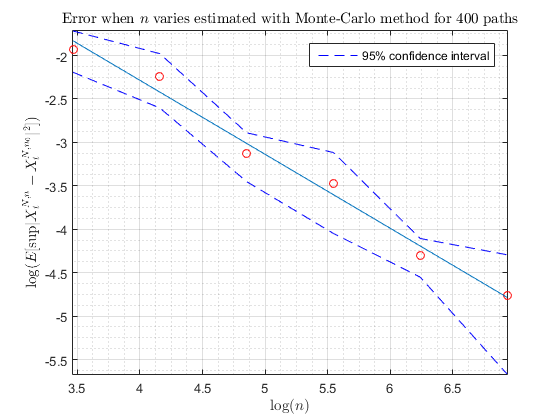
\includegraphics[width=13cm]{images/finalerror.png}
    \caption{Estimation of the $L^2$ error of the Euler-Marayuma scheme with a Monte-Carlo method. $400$ paths, $N=5$, $n\in \{2^5,2^6,2^7,2^8,2^9,2^{10}\}$, reference solution with $n_0=2^{12}$ points.}
\end{figure}

We observe a numerical strong convergence rate of $0.85$ when Theorem \ref{leo} shows a theoretical rate of $0.5-\varepsilon$.

\partb{Conclusion}

\appendix
\part{Technical proofs}

\section{Lemma \ref{local}}

As explained before, this proof is an adaptation of the one of L. Yan in \cite{Yan}. The only difference is the fact that in our case, we don't assume that the process starts at 0.
\begin{proof}[Proof of Lemma \ref{local}]
    We note $U_t(X) = \sup\{n\in\N|\tau_n<t\}$ and $n(t) = t \wedge \sigma_{U_t(X)+1}$. By Meyer-Tanaka's formula, $\forall i\in \N^*$:        
    \begin{equation}\label{tanaka}
    X^+_{\tau_i\wedge t} - X^+_{\sigma_i\wedge t} = \int_{\sigma_i\wedge t}^{\tau_i\wedge t} \mathds{1}_{\{X_s>0\}}\ \di X_s + \frac{1}{2}\left\{L^0_{\tau_i\wedge t}(X)-L^0_{\sigma_i\wedge t}(X)\right\}.
    \end{equation}        
    Because $\forall i\in\N^*,\ L^0_{\tau_{i}\wedge t}(X)=L^0_{\sigma_{i+1}\wedge t}(X)$ and $L^0_{\sigma_1\wedge t}(X)=0$, we have        
    \begin{equation*}
    \sum_{i=1}^{U_t(X)+1}\left(X^+_{\tau_i\wedge t} - X^+_{\sigma_i\wedge t}\right) = \int_{\sigma_1\wedge t}^{t} \theta_s(X)\ \di X_s + \frac{1}{2}\ L^0_{t}(X).
    \end{equation*}
    The left term is equal to $\varepsilon U_t(X)+X^+_t-X^+_{n(t)}$ so
    \begin{equation}\label{Ut}
    \varepsilon U_t(X) = \int_{\sigma_1\wedge t}^{t} \theta_s(X)\ \di X_s + \frac{1}{2}\ L^0_{t}(X) - X^+_t + X^+_{n(t)}.
    \end{equation}
    Now we express differently $U_t(X)$. $F\in\mathcal{C}^2(\R)$ so by Itô's formula:
    \begin{equation*}
    F\left(X^+_{\tau_i\wedge t}\right) - F\left(X^+_{\sigma_i\wedge t}\right) = \int_{\sigma_i\wedge t}^{\tau_i\wedge t} F'\left(X_s^+\right) \di X_s^+ + \frac{1}{2}\int_{\sigma_i\wedge t}^{\tau_i\wedge t} F''\left(X_s^+\right) \di [X^+]_s.
    \end{equation*}
    By (\ref{tanaka}), $\di X_s^+ = \mathds{1}_{\{X_s>0\}}\di X_s + \frac{1}{2}\ \di L^0_t(X)$ and $\di[X^+]_s = \mathds{1}_{\{X_s>0\}}\di[X]_s$. It follows
    \begin{multline*}
    F\left(X^+_{\tau_i\wedge t}\right) - F\left(X^+_{\sigma_i\wedge t}\right) = \int_{\sigma_i\wedge t}^{\tau_i\wedge t} F'\left(X_s^+\right) \mathds{1}_{\{X_s>0\}}\ \di X_s + \frac{1}{2}\int_{\sigma_i\wedge t}^{\tau_i\wedge t} F'(X_s^+)\ \di L^0_t(X)\\ + \frac{1}{2}\int_{\sigma_i\wedge t}^{\tau_i\wedge t} F''\left(X_s^+\right) \mathds{1}_{\{X_s>0\}}\ \di [X]_s.
    \end{multline*}
    Adding up for $i$, with $F(0) = 0$ we obtain
    \begin{multline*}
    F(\varepsilon)U_t(X)+F\left(X^+_t\right)-F\left(X^+_{n(t)}\right) = \sum_{i=1}^{U_t(X)+1} \left(F\left(X^+_{\tau_i\wedge t}\right) - F\left(X^+_{\sigma_i\wedge t}\right)\right)\\=\int_{\sigma_1\wedge t}^{ t} F'(X_s^+)\ \theta_s(X)\ \di X_s + \frac{1}{2}\int_{\sigma_1\wedge t}^{t} F'\left(X_s^+\right)\Xi_s\ \di L^0_t(X) + \frac{1}{2}\int_{\sigma_1\wedge t}^{t} F''\left(X_s^+\right)\theta_s(X)\ \di [X]_s
    \end{multline*}
    with $\Xi_s = \sum_{n=1}^\infty \mathds{1}_{\{\sigma_n<s\leq\tau_n\}}$.
    The measure $\di L^0_t(X)$ is almost surely carried by $\{t|X_t=0\}$ so we can simplify $\int_{\sigma_1\wedge t}^{t} F'\left(X_s^+\right)\Xi_s\ \di L^0_t(X) =F'(0)\int_{\sigma_1\wedge t}^{t} \Xi_s\ \di L^0_t(X)$ in order to have, with $F'(0)=0$:
    \begin{equation}\label{ito}
    F(\varepsilon)U_t(X) = - F\left(X^+_t\right) + F\left(X^+_{n(t)}\right) + \int_{\sigma_1\wedge t}^{ t} F'\left(X_s^+\right) \theta_s(X)\ \di X_s + \frac{1}{2}\int_{\sigma_1\wedge t}^{t} F''\left(X_s^+\right) \theta_s(X)\ \di [X]_s.
    \end{equation}
    Combining (\ref{Ut}) and (\ref{ito}), it follows
    \begin{multline*}
    L^0_t(X) F(\varepsilon) = 2 F(\varepsilon)(X^+_t-X^+_{n(t)})-2\varepsilon(F\left(X^+_t\right)-F\left(X^+_{n(t)}\right)\\-2\int_{\sigma_1\wedge t}^{ t} \left(F(\varepsilon) - \varepsilon F'\left(X_s^+\right)\right) \theta_s(X)\ \di X_s + \varepsilon\int_{\sigma_1\wedge t}^{t} F''\left(X_s^+\right)\theta_s(X)\ \di [X]_s.
    \end{multline*}
    Then, if $n(t) = t$, the two first right terms of the equality are equal to zero. Else, if $n(t) = \sigma_{U_t(X)+1}$, $0\leq F(\varepsilon)(X^+_t-X^+_{n(t)})=F(\varepsilon)X^+_t\leq F(\varepsilon)\varepsilon$ and $-2\varepsilon(F\left(X^+_t\right)-F\left(X^+_{n(t)}\right)=-2\varepsilon F\left(X^+_t\right)\leq0$ because of the positivity of $F$. Finally we obtain:
    \begin{equation*}
    L^0_t(X) \leq 2 \varepsilon-\frac{2}{F(\varepsilon)}\int_{\sigma_1\wedge t}^{ t} \left(F(\varepsilon) - \varepsilon F'\left(X_s^+\right)\right) \theta_s(X)\ \di X_s + \frac{\varepsilon}{F(\varepsilon)}\int_{\sigma_1\wedge t}^{t} F''\left(X_s^+\right)\theta_s(X)\ \di [X]_s.
    \end{equation*}
\end{proof}

\section{Lemma \ref{local time}}

\begin{proof}[Proof of Lemma \ref{local time}]
    By Lemma \ref{lem}, we choose $\lambda$ big enough for $\nabla u$ and $\nabla u^N$ to be bounded by $\frac{1}{2}$. $\lambda$ can be chosen independently of $N$ as far as $\norme{b - b^N}_{H_q^s(\R)} \underset{N\rightarrow\infty}{\longrightarrow} 0$. Therefore $u^N(t,\cdot)$ and $u(t,\cdot)$ are $\frac{1}{2}$-lipschitz. We recall that in this case, by Lemma 22 in \cite{Fla-Iss-Rus-2017}, $\Psi(t,\cdot)$ and $\Psi^N(t,\cdot)$ are 2-lipschitz. Therefore $\widetilde{u}^N(t,\cdot)$ and $\widetilde{u}(t,\cdot)$ are $1$-lipschitz. We can notice that $\widetilde{\nabla u}$ is $\alpha$-Hölder with constant $2^\alpha\norme{u}_{\mathcal{C}^{1,\alpha}}$ and $\nabla u^N$ is $\alpha$-Hölder with a constant which can be bounded by $\Omega$ for $N$ big enough (see Lemma 24 in \cite{Fla-Iss-Rus-2017}).
    Let $\varepsilon\in(0,1]$. Corollary \ref{cor} gives us:    
    \begin{multline*}
    0\leq L^0_T(Y-Y^N) \leq 2\varepsilon - \frac{2}{\varepsilon}\int_{\sigma_1\wedge T}^T \theta_s(Y-Y^N) \left(\varepsilon - 2{(Y_s-Y_s^N)^+}\right)\ \di \left(Y_s-Y_s^N\right)\\
    +\frac{2}{\varepsilon}\int_{\sigma_1\wedge T}^T \theta_s(Y-Y^N) \ \di\left[Y-Y^N\right]_s
    \end{multline*}    
    with
    \begin{multline*}    
    Y_T-Y_T^N = y-y^N + (\lambda + 1 )\int_0^T\left\{u\left(s,\Psi\left(s,Y_s\right)\right)-u^N\left(s,\Psi^N\left(s,Y_s^N\right)\right)\right\}\ \di s\\ + \int_0^T\left\{\nabla u\left(s,\Psi\left(s,Y_s\right)\right)-\nabla u^N\left(t,\Psi^N\left(s,Y_s^N\right)\right)\right\}\ \di W_s.
    \end{multline*}    
    \begin{rem}
        Note that $\theta_s(Y-Y^N) \left|\varepsilon - 2{(Y_s-Y_s^N)^+}\right|\leq \varepsilon\theta_s(Y-Y^N)$.
    \end{rem}    
    
    ${\nabla u}$ and ${\nabla u}^N$ are bounded so the Itô integral is a martingale. We take the expectation:
    \begin{multline*}
    \E\left[L^0_T(Y-Y^N)\right] \leq 2\varepsilon + 2(\lambda + 1)\ \E\left[\int_{\sigma_1\wedge T}^T\theta_s\left(Y-Y^N\right)\left|\widetilde{u}\left(s,Y_s\right)-\overline{u}^N\left(s,Y_s^N\right)\right| \di s \right]\\
    +\frac{2}{\varepsilon}\ \E\left[\int_{\sigma_1\wedge T}^T \theta_s\left(Y-Y^N\right)\left\{\widetilde{\nabla u}\left(s,Y_s\right)-{\overline{\nabla u}}\left(s,Y_s^N\right)\right\}^2\ \di s\right]
    \end{multline*}
    \begin{multline*}
    \leq 2\varepsilon + 2(\lambda + 1)\ \E\left[\int_0^T\theta_s\left(Y-Y^N\right)\left|\widetilde{u}\left(s,Y_s\right)-\widetilde{u}\left(s,Y_s^N\right)\right|\ \di s \right]\\+2(\lambda + 1)\ \E\left[\int_0^T\theta_s\left(Y-Y^N\right)\left|\widetilde{u}\left(s,Y_s^N\right)-\widetilde{u}^N\left(s,Y_s^N\right)\right|\ \di s \right]\\+ 2(\lambda + 1)\ \E\left[\int_{0}^T\theta_s\left(Y-Y^N\right)\left|\widetilde{u}^N\left(s,Y_s^N\right)-\overline{u}^N\left(s,Y_s^N\right)\right| \di s \right]\\
    +\frac{6}{\varepsilon}\ \E\left[\int_0^T \theta_s\left(Y-Y^N\right)\left\{\widetilde{\nabla u}\left(s,Y_s\right)-\widetilde{\nabla u}\left(s,Y_s^N\right)\right\}^2\ \di s\right]\\
    +\frac{6}{\varepsilon}\ \E\left[\int_0^T \theta_s\left(Y-Y^N\right)\left\{\widetilde{\nabla u}\left(s,Y_s^N\right)-\widetilde{\nabla u}^N\left(s,Y_s^N\right)\right\}^2\ \di s\right]\\
    +\frac{6}{\varepsilon}\ \E\left[\int_{0}^T \theta_s\left(Y-Y^N\right)\left\{\widetilde{\nabla u}^N\left(s,Y_s^N\right)-{\overline{\nabla u}^N}\left(s,Y_s^N\right)\right\}^2\ \di s\right]
    \end{multline*}
    \begin{multline*}
    \leq 2\varepsilon + 2(\lambda + 1)\ \E\left[\int_0^T\theta_s\left(Y-Y^N\right)\left|Y_s - Y^N_s\right|\ \di s \right] + 2(\lambda + 1)T\kappa\norme{b^N-b}_{H^{-\beta}_{q}} \\
    + (\lambda + 1)\ \E\left[\int_{0}^T\theta_s\left(Y-Y^N\right)\left|\Psi\left(s,Y_s^N\right)-\Psi^N\left(s,Y_s^N\right)\right| \di s \right]\\  
    +\frac{6\times4^{\alpha}\norme{u}_{\mathcal{C}^{1,\alpha}}^2}{\varepsilon}\ \E\left[\int_0^T \theta_s\left(Y-Y^N\right)\left|Y_s - Y^N_s\right|^{2\alpha}\ \di s\right]  + 6T\kappa^2\norme{b^N-b}_{H^{-\beta}_{q}}^2\varepsilon^{-1} \\+\frac{6\Omega^2}{\varepsilon}\ \E\left[\int_{0}^T \theta_s\left(Y-Y^N\right)\left|\Psi\left(s,Y_s^N\right)-{\Psi^N}\left(s,Y_s^N\right)\right|^{2\alpha}\ \di s\right]\\
    \end{multline*}
    where we have used Lemma \ref{morrey}, the $1$-lipschitz property of $\widetilde{u}$, the $1/2$-lipschitz property of $u^N$, the $\alpha$-Hölder property of $\widetilde{\nabla u}$ (with constant $2^\alpha\norme{u}_{\mathcal{C}^{1,\alpha}}$), and the $\alpha$-Hölder property of $\nabla u^N$ (with constant $\Omega$). Lemma \ref{psi} gives us:
    \begin{multline*}
    \leq 2\varepsilon + 2(\lambda + 1)\ \E\left[\int_0^T\theta_s\left(Y-Y^N\right)\left|Y_s - Y^N_s\right|\ \di s \right] + 4(\lambda + 1)T\kappa\norme{b^N-b}_{H^{-\beta}_{q}} \\  
    +\frac{6\times4^{\alpha}\norme{u}_{\mathcal{C}^{1,\alpha}}^2}{\varepsilon}\ \E\left[\int_0^T \theta_s\left(Y-Y^N\right)\left|Y_s - Y^N_s\right|^{2\alpha}\ \di s\right]+ 6T\kappa^2\norme{b-b^N}_{H^{-\beta}_{q}}^2\varepsilon^{-1}\\   + 6\Omega^2T4^{\alpha}\kappa^{2\alpha} \norme{b-b^N}_{H^{-\beta}_q}^{2\alpha}\varepsilon^{-1}.
    \end{multline*}
    As $\theta_s(Y-Y^N)\left|Y_s - Y^N_s\right|\leq \varepsilon$, we have    
    \begin{multline*}
    \E\left[L^0_T(Y-Y^N)\right]\leq 2\varepsilon + 2(\lambda + 1)\ T\varepsilon
    +4(\lambda + 1)T\kappa\norme{b-b^N}_{H^{-\beta}_{q}}+6\norme{u}_{\mathcal{C}^{1,\alpha}}^2 4^{\alpha}T \varepsilon^{2\alpha-1} \\ + 6T\left(\Omega^24^{\alpha}\kappa^{2\alpha} \norme{b-b^N}_{H^{-\beta}_q}^{2\alpha}+\kappa^2\norme{b-b^N}_{H^{-\beta}_{q}}^2\right)\varepsilon^{-1}.
    \end{multline*}    
    As $1>2\alpha-1>0$, the result follows from $\varepsilon\leq\varepsilon^{2\alpha-1}$ when $0<\varepsilon\leq1$.  
    
\end{proof} 

\section{Lemma \ref{key lemma}}

\begin{proof}[Proof of Lemma \ref{key lemma}]
    Let $\varepsilon\in(0,1]$, by Lemma \ref{local time},    
    \begin{equation*}
    0\leq\E\left[L^0_T(Y-Y^N)\right]\leq g(\varepsilon)
    \end{equation*}
    where \begin{multline*}
    g(\varepsilon) = 4(\lambda + 1)T\kappa\norme{b-b^N}_{H^{-\beta}_{q}} + \left(2 + 2(\lambda + 1)\ T + 6\norme{u}_{\mathcal{C}^{1,\alpha}}^2 4^{\alpha}T\right) \varepsilon^{2\alpha-1} \\ + 6T\left(\Omega^24^{\alpha}\kappa^{2\alpha} \norme{b-b^N}_{H^{-\beta}_q}^{2\alpha}+\kappa^2\norme{b-b^N}_{H^{-\beta}_{q}}^2\right)\varepsilon^{-1}.
    \end{multline*}    
    With \begin{multline*}
    g'(\varepsilon)=(2\alpha-1)\left(2 + 2(\lambda + 1)\ T + 6\norme{u}_{\mathcal{C}^{1,\alpha}}^2 4^{\alpha}T\right)\varepsilon^{2\alpha-2}\\-6T\left(\Omega^24^{\alpha}\kappa^{2\alpha} \norme{b-b^N}_{H^{-\beta}_q}^{2\alpha}+\kappa^2\norme{b-b^N}_{H^{-\beta}_{q}}^2\right)\varepsilon^{-2},
    \end{multline*}
    and 
    \begin{multline*}
    g''(\varepsilon)=(2\alpha-2)(2\alpha-1)\left(2 + 2(\lambda + 1)\ T + 6\norme{u}_{\mathcal{C}^{1,\alpha}}^2 4^{\alpha}T\right)\varepsilon^{2\alpha-3}\\+12T\left(\Omega^24^{\alpha}\kappa^{2\alpha} \norme{b-b^N}_{H^{-\beta}_q}^{2\alpha}+\kappa^2\norme{b-b^N}_{H^{-\beta}_{q}}^2\right)\varepsilon^{-3},\end{multline*}
    
    the minimum of $g$ on $(0,1]$ is reached when $N$ is big enough in \begin{equation*}
    \varepsilon_N=\left(\frac{6T\left(\Omega^24^{\alpha}\kappa^{2\alpha} \norme{b-b^N}_{H^{-\beta}_q}^{2\alpha}+\kappa^2\norme{b-b^N}_{H^{-\beta}_{q}}^2\right)}{(2\alpha-1)\left(2 + 2(\lambda + 1)\ T + 6\norme{u}_{\mathcal{C}^{1,\alpha}}^2 4^{\alpha}T\right)}\right)^{\frac{1}{2\alpha}}=\omega_N \norme{b^N-b}_{H^{-\beta}_{q}}.
    \end{equation*}
    
    where 
    \begin{equation*}
    g''(\varepsilon_N)
    =12T\left(\Omega^24^{\alpha}\kappa^{2\alpha} +\kappa^2\norme{b-b^N}_{H^{-\beta}_{q}}^{2(1-\alpha)}\right)\varepsilon_N^{-3}\alpha>0.
    \end{equation*}
    
    and \begin{equation*}
    \omega_N = \left(\frac{6T\left(\Omega^24^{\alpha}\kappa^{2\alpha} +\kappa^2\norme{b-b^N}_{H^{-\beta}_{q}}^{2(1-\alpha)}\right)}{(2\alpha-1)\left(2 + 2(\lambda + 1)\ T + 6\norme{u}_{\mathcal{C}^{1,\alpha}}^2 4^{\alpha}T\right)}\right)^{\frac{1}{2\alpha}}
    \end{equation*}
    \begin{equation*}
    \geq\omega_\infty=\left(\frac{6T\Omega^24^{\alpha}\kappa^{2\alpha} }{(2\alpha-1)\left(2 + 2(\lambda + 1)\ T + 6\norme{u}_{\mathcal{C}^{1,\alpha}}^2 4^{\alpha}T\right)}\right)^{\frac{1}{2\alpha}}.
    \end{equation*}
    
    Therefore $
    \E\left[L^0_T(Y-Y^N)\right]\leq g(\varepsilon_N)
    $
    \begin{multline*}
    \leq 4(\lambda + 1)T\kappa\norme{b-b^N}_{H^{-\beta}_{q}} + \left(2 + 2(\lambda + 1)\ T + 6\norme{u}_{\mathcal{C}^{1,\alpha}}^2 4^{\alpha}T\right) \omega_N^{2\alpha-1}\norme{b-b^N}_{H^{-\beta}_{q}}^{2\alpha-1} \\ + 6T\left(\Omega^24^{\alpha}\kappa^{2\alpha} \norme{b-b^N}_{H^{-\beta}_q}^{2\alpha}+\kappa^2\norme{b-b^N}_{H^{-\beta}_{q}}^2\right)\omega_N^{-1}\norme{b-b^N}_{H^{-\beta}_{q}}^{-1}
    \end{multline*} 
    \begin{multline*}
    \leq 4(\lambda + 1)T\kappa\norme{b-b^N}_{H^{-\beta}_{q}} + \left(2 + 2(\lambda + 1)\ T + 6\norme{u}_{\mathcal{C}^{1,\alpha}}^2 4^{\alpha}T\right) \omega_N^{2\alpha-1}\norme{b-b^N}_{H^{-\beta}_{q}}^{2\alpha-1} \\ + 6T\left(\Omega^24^{\alpha}\kappa^{2\alpha} +\kappa^2\norme{b-b^N}_{H^{-\beta}_{q}}^{2(1-\alpha)}\right)\omega_\infty^{-1}\norme{b-b^N}_{H^{-\beta}_{q}}^{2\alpha-1}
    \end{multline*}   
    \begin{multline*}
    \leq 4(\lambda + 1)T\kappa\norme{b-b^N}_{H^{-\beta}_{q}}^{2\alpha-1} + \left(2 + 2(\lambda + 1)\ T + 6\norme{u}_{\mathcal{C}^{1,\alpha}}^2 4^{\alpha}T\right)2 \omega_\infty^{2\alpha-1}\norme{b-b^N}_{H^{-\beta}_{q}}^{2\alpha-1} \\ + 6T\left(\Omega^24^{\alpha}\kappa^{2\alpha} +\kappa^2\right)\omega_\infty^{-1}\norme{b-b^N}_{H^{-\beta}_{q}}^{2\alpha-1}
    \end{multline*}
    for $N$ big enough. The result follows.
\end{proof}

\listoffigures

\bibliographystyle{abbrv}
\bibliography{pre}

\end{document}